
\clearpage
%\doublespacing
\section{Results and discussion}

	\subsection{Conserved residues within NS1 bind dsDNA and control transcription of cellular genes (Study I)}
	
		The nucleic acid binding function of NS1 is extremely important for influenza A replication and residues R38 and K41 are conserved across viral subtypes \parencite{Hatada1992, Zohari2008}. The mutations R38A and K41A were shown to prevent dsRNA binding by NS1, and result in increased IFN production by infected cells and severely attenuated viral phenotype \parencite{Donelan2003}. Although the proposed role of nucleic acid binding by NS1 is sequestration of viral replication intermediates away from cellular \gls{PRR}s, it is controversial as discussed Section \ref{sec:pre-transcriptional}. We addressed the role of nucleic acid binding function of NS1 using the recombinant influenza A/WSN/33 (WSN) viruses expressing \gls{wt} NS1 or its R38A, K41A (RK/AA) mutant which can not bind nucleic acids. In agreement with previous studies \parencite{Min2006}, RK/AA WSN virus exhibited severely attenuated phenotype in cell culture. 
		
		Gene expression profiling of human macrophages infected with RK/AA viruses resulted in strong up-regulation of a large set of cellular genes (\textbf{I}, fig. 1A and B). Gene set enrichment analysis \parencite{Subramanian2005} indicated that these genes were involved in the regulation of innate and adaptive immune responses and belonged to TLR and Jak/STAT signaling pathways, cytokine-cytokine receptor interaction and natural killer cell mediated cytotoxicity pathways. Accordingly, RK/AA infection resulted in increased production of both antiviral and pro-inflammatory cytokines (\textbf{I}, fig. 1C). Importantly, the effect of RK/AA mutations on cellular gene expression and cytokine production was not specific to immune cells and was also observed in a retinal pigment epithelium (RPE) cell line (\textbf{I}, suppl. fig. 1A and B). 
		
		Wild type NS1 is abundant in the insoluble fraction of cell lysate (\textbf{I}, 2A), where it associates with cellular chromatin, presumably via protein-DNA, protein-protein or both interactions (\textbf{I}, 2B). Although the direct binding of NS1 to dsDNA has not been shown previously, the structure of NS1 RBD and full-length dimer does not exclude its interaction with dsDNA \parencite{Bornholdt2008, Cheng2009}. Therefore, we tested this possibility in an \gls{EMSA} using purified recombinant \gls{wt} and RK/AA NS1 proteins and synthetic DNA. Indeed, purified wild-type NS1 did interact with 190 bp long linear dsDNA and the \gls{Kd} was 11.1~$\pm$~0.7~ $\mu$M, indicative of a probably nonspecific binding. The residues R38 and K41 were absolutely required for dsDNA interaction (\textbf{I}, fig. 3B, C). 
		
		The ability of NS1 to associate with cellular chromatin and to bind dsDNA prompted us to test its effects on transcription. To dissect effects of  NS1-dsDNA binding and upstream events we addressed this question in a cell-free run-off transcription assay using purified \gls{wt} and RK/AA NS1 proteins. Binding of wt NS1 to DNA had inhibitory effects on RNA synthesis by RNA polymerase II and time of addition experiment suggested that NS1 inhibited transcription at its initiation step (\textbf{I}, fig. 3D, E). Interestingly, NS1 prevented RNA synthesis after preincubation  with dsDNA or with transcription factors and RNA polymerase II (\textbf{I}, fig. 3F). This finding indicates that NS1 binds dsDNA and inhibits transcription initiation by preventing pre-initiation complex and RNA polymerase II loading on dsDNA. Alternatively, dsDNA binding could coordinate inhibitory protein-protein interactions between NS1 and components of transcription initiation machinery. 
		
		Is the dsDNA binding by NS1 that we observed \textit{in vitro} relevant to infection? To answer this question we addressed NS1 interaction with dsDNA in infected cells. \Gls{ChIP} experiment in infected cells revealed the presence of NS1 on the promoter and exon regions of the \textit{IFNB1} gene which is strongly induced upon influenza A infection. Interaction of NS1 with \textit{IFNB1} DNA was R38-, K41-dependent, suggesting direct dsDNA binding as was observed in an \textit{in vitro} assay (\textbf{I}, fig. 4A). The pattern of NS1 association with \textit{IFNB1} promoter and exon regions was opposite to that of RNA polymerase II, which may indicate possible inhibition of \textit{IFNB1} gene expression due to NS1 DNA-binding. 
		
		Functional versatility of NS1 complicates studying the role of its dsDNA binding in the context of viral infection, as in addition to nucleic acid binding residues R38 and K41 are involved in inhibitory interactions with TRIM25, RIPLET and \gls{RIG-I}, which also prevent transcriptional activation of \textit{IFNB1} \parencite{Gack2009, Rajsbaum2012}. To split NS1 transcriptional effects from its role in virus-induced \gls{RIG-I} signaling, we addressed the function of its R38 and K41 in transfected cells overexpressing NS1. In this system NS1 was also able to interact with cellular DNA as we detected it on promoter and exon of housekeeping gene \textit{EML4} (\textbf{I}, fig. 4C). We addressed direct effects of NS1 dsDNA binding on transcriptional regulation of cellular genes by exposing transfected cells to \gls{polyic}. External \gls{polyic} is detected by cell surface \gls{TLR}3  and thus \gls{IFN} responses are induced without activation of dsRNA signaling \parencite{Karpala2005}. As expected, NS1 capable of dsDNA binding strongly inhibited \gls{polyic}-induced activation of \textit{IFNB1}, \textit{IFNA1} and \textit{IFNA16}, supporting our hypothesis of its role in direct transcriptional inhibition (\textbf{I}, fig. 4D).
		
		In summary, these results provide a novel insight into IFN responses control by NS1, suggesting direct binding of NS1 to promoter and exon regions DNA and prevention of effective transcription of cellular genes. The \gls{Kd} of NS1-dsDNA binding was 11.1~$\pm$~0.7~ $\mu$M and is comparable to the \gls{Kd} of NS1-dsRNA binding, which is also in micromolar range \parencite{Yin2007}. Provided this, and also given that the \gls{NS1} is predominantly localized in cellular nucleus, where its concentration is very high \parencite{Li2010, Marazzi2012}, we can propose that the dsDNA-binding  of NS1 is as important as its well-described dsRNA-binding. Further studies in \gls{RIG-I}-, \gls{PKR}- and \gls{OAS}-deficient systems would be helpful for dissecting these two essential functions of NS1. 
		
		From our studies we can not determine, whether NS1 interacts with dsDNA as a dimer or as an oligomer. Interestingly, the tunnel diameter inside the NS1 oligomer was reported to be 20 \gls{A} \parencite{Bornholdt2008}, and, if no conformational changes occur during binding, it is more likely to accommodate a 20 \gls{A} B-form DNA double helix, rather than 26 \gls{A} RNA double helix. This question could be addressed in detail with further biophysical and structural studies of NS1-dsDNA complex.
		
		With regards sequence specificity of NS1 dsNDA binding, our results suggest the lack of it, however, one can speculate that during infection transcriptionally active chromatin, i.e. \textit{IFN} genes, is more accessible to NS1. This question, however, needs to be addressed in detail using genome-wide studies, for example, \gls{ChIP} combined with sequencing. Furthermore, our \textit{in vitro} results suggest that NS1 is able to bind dsDNA \textit{per se}, however it would be interesting to investigate whether NS1 interacts with possible cellular factors to facilitate its targeting to dsDNA in a crowded nucleus environment.
		
		When this study was initiated, NS1 had been thought to control activation of antiviral genes at pre-transcriptional level (see section \ref{sec:pre-transcr}). However, later it was shown that NS1 also inhibits cellular transcription by targeting histone H3-interacting transcription elongation complex PAF1 \parencite{Marazzi2012}. Such an inhibition, however, required histone-mimic sequence \textsuperscript{226}ARSK\textsuperscript{229} in NS1 C-terminus and was specific to viruses of H3N2 subtype \parencite{Marazzi2012}. The mechanism of transcriptional control by NS1 discovered in our study, in contrast, seems to be general across different influenza A subtypes and involves conserved residues R38, K41. The importance of NS1 dsDNA binding for viral replication and conservation of R38 and K41 suggest that this function of NS1 could be an interesting target for antivirals development. Indeed, a recent study utilized SELEX approach to select ssDNA aptamers that are bound by NS1 with high affinity and suppress its anti-interferon functions \parencite{Woo2013}.
											
						
	\subsection{Regulation of general protein synthesis by NS1 (Studies II, IV)}
	
		Another essential function of NS1 is to support effective viral protein synthesis in the context of infection and thus secure viral replication. Influenza A infection activates cellular \gls{PKR} which phosphorylates and inactivates translation initiation factor \gls{eIF2a}, thus inhibiting protein synthesis and inducing death of infected cells \parencite{Levin1978}. NS1 regulates general protein synthesis by preventing  \gls{PKR} activation and its residues 123--127 are thought to be essential for this \parencite{Lu1995, Min2007}. In addition, NS1 interacts with translation initiation factors \gls{eIF4GI} and \gls{PABP}I and some studies proposed that it recruits these factors to viral mRNAs thus specifically enhancing viral protein synthesis \parencite{DelaLuna1995, Aragon2000, Burgui2003}. Such recruitment, however, would require specific binding of NS1 to distinct sequences on viral mRNAs.
		
		We addressed regulation of protein synthesis by NS1 and to separate the effects of NS1 on protein synthesis from its other functions we used a \gls{RRL} cell-free translation system. 
		
		Avian high pathogenic H5N1 NS1 enhanced translation of reporter mRNA and protein production by \gls{RRL} over 6 fold (\textbf{II}, fig. 2A and C). Importantly, the RNA-binding function of NS1 was not required for translation regulation in \gls{RRL} and the RK/AA mutant protein was as efficient enhancer of translation as the \gls{wt} (\textbf{II}, fig. 2A). This observation allowed us to use the RK/AA NS1 proteins in further experiments as they show remarkably better solubility compared to the \gls{wt} \parencite{Bornholdt2008}. 
		
		NS1 effects on translation in \gls{RRL} were subtype specific: avian H5N1 and H5N2 NS1s were efficient translational enhancers, whereas pH1N1/2009 NS1 did not affect protein synthesis (\textbf{II}, fig. 2B and C). 
		
		Translational enhancement by NS1 was not limited to viral mRNAs. In \gls{RRL} programmed with RNAs extracted from infected cells at different time points post infection NS1 enhanced production of both viral and cellular proteins (\textbf{IV}, fig. 1A). This finding was supported by  our observation that NS1 RNA-binding was not required for its translational control in \gls{RRL}. 
		
		In addition to its interactions with translation factors, NS1 has been shown to associate with \gls{hStau} on polysomes in infected cells \parencite{Falcon1999}. As the \gls{hStau} has been implicated in regulation of mRNA stability, we addressed if translational enhancement in \gls{RRL} in the presence of \gls{NS1} was a result of increased mRNA stability. This appeared not to be the case and NS1 did not affect the mRNA degradation rate (\textbf{II}, fig. 2E and F). Instead, NS1 enhanced association of mRNA with ribosomes and polysomes in RRL reactions which suggested its possible role in translation initiation (\textbf{IV}, fig. 1B).
		
		We utilized differential effects of H5N1, H5N2 and pH1N1/2009 NS1 proteins on RRL protein synthesis to map NS1 residues essential for translation enhancement. The NS1 protein of pH1N1/2009 is 11 \gls{aa} shorter than H5N1 and H5N2 \glspl{NS1} due to a C-terminal truncation. However, neither 11 C-terminal residues, nor the whole \gls{ED} was essential for translation modulation by \gls{NS1}. RBD alone was sufficient for this function (\textbf{II}, fig. 2G and H). The RBD of pH1N1/2009 NS1 contained several unique amino acids compared to H5N1 and H5N2: N25, G26, N48 and W67 (\textbf{II}, fig. 1A). Introduction of these residues singularly or all at once into H5N1 NS1 resulted in loss of its function in RRL protein synthesis. In a reciprocal experiment introduction of Q25/N26 and R67 from H5N1 in pH1N1/2009 NS1 resulted in its gain of function confirming that these residues are essential for translational control in RRL (\textbf{II}, fig. 2I). The side chains of these amino acids are exposed to solvent, indicating their possible involvement in interaction between NS1 and its protein partner (\textbf{II}, fig. 4B). Thus, we found that in \gls{RRL} NS1 non-specifically enhances production of both viral and cellular proteins and critical residues for this function are Q25, E26, S48 and R67 with \gls{NS1} \gls{RBD}.
		
		In the system that we used, the stimulation of protein synthesis in \gls{RRL} was not specific to viral mRNAs and also did not require NS1 RNA-binding function. Therefore, this approach can not address the ability of NS1 to target translation factors to viral mRNAs and our data neither contradict, nor support previous studies. Translational enhancement by NS1 in RRL occurred due to prevention of \gls{eIF2a} phosphorylation (Fig. \ref{fig:WB}). 
		
			\begin{figure}[h!]
				\centering
				\fbox{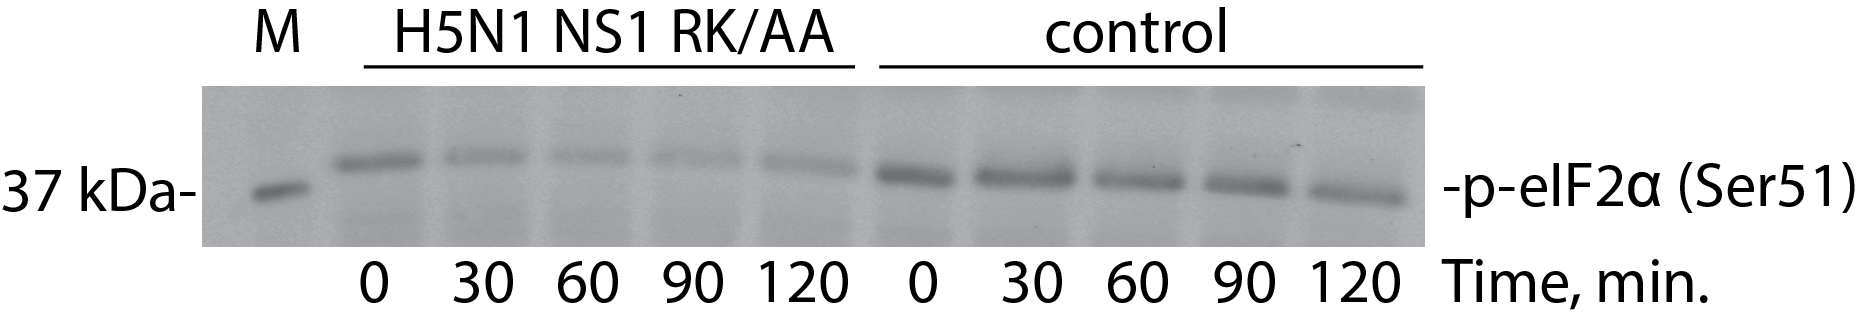
\includegraphics[width=0.5\textwidth]{WB_RRL2.png}}
				\caption{NS1 inhibits \gls{eIF2a} phosphorylation in \gls{RRL}. RRL reactions were supplied with H5N1 RK/AA NS1 or control buffer and incubated for the time indicated. Equal amounts of reaction mixes were loaded on the SDS-polyacrylamide gel and phosphorylation status of \gls{eIF2a} was assayed using immunoblot.} \label{fig:WB}
			\end{figure}
		
		There are four kinases that can phosphorylate \gls{eIF2a}: \gls{PKR}, \gls{PERK}, \gls{GCN2} and \gls{HRI} \parencite{Donnelly2013}. Of these, only \gls{PKR} has an assigned role in influenza infection. NS1 is proposed to prevent activation of the \gls{PKR} by two mechanisms: (i) by binding to dsRNA with its R38 and K41 and sequestering it away from \gls{PKR} \parencite{Lu1995} or (ii) by direct interaction with \gls{PKR} via its residues 123--127 \parencite{Min2007} and the latter activity is proposed to be critical for \gls{PKR} inactivation. It is possible that endogenous \gls{PKR} is activated in \gls{RRL} and \gls{NS1} prevents this activation thus securing protein synthesis. However, three observations are not in line with this mechanism: (i) RNA-binding function of NS1 was not required for its function in \gls{RRL}. Therefore, NS1 prevented \gls{eIF2a} phosphorylation probably not by sequestering possible dsRNA substrates of PKR; (ii) our data indicates that only \gls{NS1} \gls{RBD} is sufficient to prevent \gls{eIF2a} phosphorylation in RRL via its residues Q25, E26, S48 and R67, whereas previously published data suggests that PKR inhibition by NS1 requires \glspl{aa} 123--127; and (iii) a previous study by Min et al. reported that \gls{RBD} of A/Udorn/72 H3N2 which is highly similar to H5N1 and H5N1 NS1 \glspl{RBD} and contains residues Q25, E26, S48 and K67 did not inhibit \gls{PKR} \parencite{Min2007}. Therefore, it is possible that the protein partner of NS1 in \gls{RRL} is \gls{PKR}. The other possible kinases that could be inhibited by \gls{NS1} are \gls{HRI}, \gls{GCN2} and \gls{PERK}. Although the role of these kinases in influenza A infection is not known,  all of them are induced in response to various stress stimuli \parencite{Donnelly2013}. The possible inhibition of one of these proteins by \gls{NS1} could represent an additional approach by which influenza A secures protein synthesis during cellular stress. However, the exact target of NS1 is yet to be identified. 

		Because NS1 proteins used in our work were deficient of RNA binding, our results do not address possible targeting of NS1 on specific sequences on mRNA. However, in a recent study Marc et al. have identified virus-specific motifs on RNAs to which NS1 bound with nanomolar \gls{Kd} \parencite{Marc2013}. Biologically, such binding could be related to several essential processes in virus life cycle, including enhanced translation of viral mRNAs, however, it is still yet to be confirmed in infected cells. Altogether, our results do not contradict possible targeting of NS1 to viral mRNAs, but demonstrate a strategy of general protein synthesis stabilisation during infection employed by the virus. 
		
	\subsection{C-terminus of NS1 contributes to modulation of host antiviral responses (Study III)}
		
		Although NS1 is a well structured protein, its C-terminus is likely to be unstructured \parencite{Hale2008b}. Nevertheless, it can play an essential regulatory role in infection, as it accommodates numerous interaction motifs and modification sites that can modulate virus-host interactions, ofter in strain-specific manner \parencite{Liu2010, Marazzi2012, Li2001, Melen2012, Hsiang2012, Hsiang2009}. Naturally occurring truncations and extensions of NS1 C-terminus are not uncommon \parencite{Suarez1998}. The NS1 protein of H1N1 viruses isolated in 2009--2014 is typically 219 aa long, H1N1 viruses encoding NS1 of 202 and 230 aa have been recently reported in Finnish patients \parencite{Lakspere2014}. However, the relevance of NS1 C-terminal truncations and extensions to viral replication and virulence is unclear.
		
		We aimed to address the functional role of NS1 C-terminus length using influenza A viruses of well-characterized A/WSN/33 background that express NS1 proteins of 202, 220 and 230 amino acids (\textbf{III}, fig. 1B). All viruses were able to propagate in immune-competent MDCK cells, but the virus with the shortest NS1 (202 \gls{aa}) displayed delayed growth kinetics (\textbf{III}, suppl. fig. 1A). 
		
		We addressed the effects of NS1 C-terminus length in human macrophages. Sequential truncations of NS1 C-terminus increased transcriptional activation of cellular genes and the virus expressing the shortest NS1 was least successful in control of host gene expression (\textbf{III}, 2A). The majority of genes, differentially regulated by NS1 C-terminus length, e.g. \textit{MX1}, \textit{ISG15}, \textit{OASL}, \textit{CCL8}, \textit{IL6}, and \textit{IL8}, was involved in the regulation of innate and adaptive immune responses (\textbf{III}, fig. 2B).  This effect was to some extent reflected on the level of cytokine secretion and amounts of IL-6 and IL-8 secreted by macrophages were increased upon NS1 truncations (\textbf{III}, fig. 2C and D). 
		
		Differential regulation of immune-related gene expression and cytokine production prompted us to address the role of the NS1 C-terminus in cellular signaling pathways. We observed that C-terminal truncations of NS1 upregulated phosphorylation of several phosphoproteins involved in control of immune responses. The shorter the NS1 C-terminus was, the stronger was observed phosphorylation of STAT3, JNK, HSP60 and AMPK$\alpha$1 (\textbf{III}, fig. 3). 
				
		We used the viruses that express 230 and 202 aa long NS1 to address the effect of NS1 C-terminus \textit{in vivo}. NS1 C-terminus deletion reduced influenza A virulence and pathogenicity in mice (\textbf{III}, fig. 4A and B), suggesting the regulatory role of NS1 C-terminus in infection. Thus, our results indicate that the length of NS1 C-terminus is essential for interactions with the host cell, control of antiviral responses and modulation of viral pathogenicity. 
		
		The C-terminus of A/WSN/33 NS1 contains human-like PDZ-binding motif for which no interactions have yet been identified and a phosphorylation site T215 for which the effect is also unclear \parencite{Jackson2010, Hsiang2012}. Nevertheless, our data indicate the functional role of NS1 C-terminus length in the regulation of the host immune responses and in viral pathogenicity and virulence. Sporadic truncations and extensions of NS1 are quite seldom events, but they could provide opportunities to lose, acquire or activate functional motifs within NS1 C-terminus. For example, despite in initial experiments appearance of functional Crk/CrkL-binding motif in H1N1 NS1 C-terminus did not bring on notable effects \parencite{Hale2010e}, it seems that a combination of Crk/CrkL and NS1 C-terminus extension do increase viral replication and virulence (Dr. Eike Hrincius, personal communication) and further modeling of C-terminal polymorphisms on pH1N1/2009 genetic background could provide deeper insights in virus-host interactions and influenza A adaptation to host.
		
		The H1N1 influenza A viruses isolated from 2009 demonstrate the highest substitution rate in NS1 compared to other known viral subtypes \parencite{Xu2011}. A recent study conducted in UK indeed reported that currently circulating pH1N1/2009 virus rapidly adapts to human, and acquires mutations in multiple viral genes, including NS1, that increase viral replication and limit host cytokine production \parencite{Elderfield2014}. Several isolates of pH1N1/2009 influenza A have acquired a functional Crk/CrkL-binding domain or an extended C-terminus (\textbf{III}, fig. 1A). Although such viruses may not be of immediate concern, monitoring of changes within NS1 and its C-terminus is worth undertaking, as while amino acid variations in NS1 C-terminus are not detrimental, they provide opportunity for the influenza A to probe additional ways of virus-host interactions under human selection pressure.
		
		%Our observation that the virus expressing NS1 protein lacking C-terminus induced stronger antiviral responses and demonstrated attenuated phenotype in immune-competent systems suggests that such viruses could be also studies as attractive vaccine candidates.
		 
	
	\subsection{NS1 as a tool to improve cell-free protein synthesis system (Study IV)}
	
		The effects of NS1 on translation in \gls{RRL} observed in Study II prompted us to utilize NS1 for improvement of \gls{RRL} cell-free translation system. \gls{RRL} is widely used for translation of specific templates, membrane protein studies, post-translational events in folding and protein modification, and high-throughput screening for protein-protein interactions \parencite{Fuller2000, Douthwaite2012, Fixsen2010, Wang2011}. However, low protein yield is a considerable limitation of RRL, which should be overcome to improve its current applications \parencite{Carlson2012}. As viruses have evolved multiple ways to facilitate protein synthesis, a possible way to improve cell-free protein synthesis is addition of viral factors which regulate translation. These include viral proteins and specific regulatory structures on mRNA such as \gls{UTR}s or \glspl{IRES}. 
	
		The NS1-mediated enhancement of \gls{RRL} translation occurred through inhibition of \gls{eIF2a} phosphorylation (fig. \ref{fig:WB}) and stabilization of translation initiation and was not specific to viral mRNAs (\textbf{IV}, fig. 1). We reasoned that \gls{RRL} translation could be reinforced using mRNAs with specific 5' and 3' regulatory structures which together with \gls{NS1} would exert a cumulative effect. For this several reporter mRNAs with \gls{5meG} or \gls{IRES} and with different 3' \gls{UTR}s were tested in RRL at their optimal concentration (\textbf{II}, fig. 2D; \textbf{IV}, fig. 2A). We observed the most robust enhancement of translation when mRNA containing 5' \gls{EMCV} \gls{IRES} and 3' \gls{polyA} sequence was used together with NS1. The protein production by RRL in this case was increased over 11 times (\textbf{IV}, fig. 2B). The \gls{EMCV} \gls{IRES} is known to initiate translation with limited initiation factors requirement and without ribosome scanning for AUG codon \parencite{Pestova2001}. However, it is still dependent on non-phosphorylated \gls{eIF2a} \parencite{Terenin2008}, which in our system is controlled by NS1. 
	
		In summary, our strategy to use viral enhancers of translation provides an easy and efficient way to improve cell-free translation in \gls{RRL} and enhance its protein yield. This strategy appears to be more effective compared to traditional usage of small molecular inhibitors of \gls{eIF2a} kinases \parencite{Jammi2003}. It also provides a proof-of-concept for generally utilizing viral proteins to modify cell-free translation systems from different origins.
	
\newpage
\section{Conclusions and future perspectives}

		NS1 is an extremely versatile protein that controls influenza A virus-host interactions at multiple levels. It has been extensively studied over the past few decades, but despite a great deal of information has been obtained, the understanding of multiple functions of NS1 is still far from  completeness. For example, nucleic binding by R38 and K41 of NS1 has been well-described, but its role in the viral replication cycle still needs elucidation (section \ref{sec:pre-transcriptional}). NS1 interactions with cellular factors of translation might facilitate selective synthesis of viral proteins, but the exact mechanism needs to be described (section \ref{sec:pro-viral}). Furthermore, a C-terminal disordered ``tail'' of NS1 is a key contributor to NS1 diversity and length polymorphisms, but its role in viral replication is far from being understood (section \ref{sec:diversity}).
		
		In this work I set few specific questions aiming to provide novel insights into modulation of influenza A virus-host interactions by NS1: What is the role of NS1 nucleic acid binding and residues R38 and K41 in infection? Does NS1 specifically or non-specifically enhance translation? What is the contribution of NS1 C-terminus in modulation of virus-host interactions? 
		
		We approached of nucleic acid binding by NS1 in our study I and demonstrated that NS1 can directly bind dsDNA and inhibit cellular gene expression at transcriptional level. It does not exclude the RNA-binding, bu seems to be as important and provides additional level of NS1 control over host immune responses. As it often occurs in science, our observation not only uncovers a previously undescribed function of NS1, but also brings up several questions for further elucidation. 
		
		How does NS1 inhibit transcription in the cell, without leading to its premature death? Does it target specific cellular gene subsets? Are there any cellular factors hijacked by the virus to secure this targeting? Addressing these questions in genome-wide distribution of NS1 on cellular dsDNA using a high throughput method such as ChIP-seq, and identification of NS1 interaction partners using immunoprecipitation coupled with mass-spectrometry analysis could contribute to understanding the mechanistic details of transcriptional control by NS1. As the NS1 residues involved in this function are conservative, one would expect that the transcriptional control by dsDNA binding is a common function of NS1 proteins. Is it so? This can be addressed in question in similar studies using other influenza A viruses, such as A/Udorn/72 (H3N2), A/PR8/34 (H1N1) and A/California/07/2009 (pH1N1/2009) for which reverse genetics systems are available. Furthermore, as the NS1 nucleic acid binding function(s) appear to be critical for influenza A replication in immune competent systems and residues R38 and K41 are conserved, targeting this function with an inhibitor molecule may provide a promising antiviral, to which resistance is less likely to be developed.
		
		In our study II we addressed the translation modulation by NS1 in a cell-free translation system. We observed that NS1 non-specifically enhanced translation of viral and cellular mRNAs. The mapped the residues within NS1 that secure this function indicate that this function occurs via protein-protein interactions and RNA-binding function is not involved. Thus, our results did not disprove or support previous suggestions that NS1 specifically targets viral mRNAs and recruits translation factors there. But we rather added a new level  of translational control by NS1. Although our studies of translational control by NS1 might be limited by the system used, our results provoke further investigation of cellular responses to influenza A infection. Are there translational regulators, other than PKR, induced by viral infection and accompanied cellular stress? Answering this question by specific studies of other eIF2$\alpha$ kinases activation upon influenza A infection and probing possible protein-protein interactions between NS1 and these kinases can bring new insights in understanding of complex control over cellular protein synthesis during infection.
		
		Interestingly, our observation that NS1 prevents eIF2$\alpha$ phosphoylation in RRL allowed us to develop an approach to utilize NS1 to improve biotechnologically important cell-free translation system and increase its protein yield. Our study IV has laid a proof of principle for using viral translational enhancers in biotechnological systems. As Influenza A infects birds and mammals, our method improved mammalian cell-free translation system based on \gls{RRL}. Viruses infect all forms of life and are obligate parasites of host translation, hence further studies may identify viral enhancers for any given cell-free translation system.
		
		Finally, in our study III we showed that the length of NS1 C-terminal tail contributes to control over cellular antiviral responses and regulates virus pathogenicity. These findings suggests that further monitoring of NS1 length polymorphisms should be undertaken. As the majority of human influenza A infections is currently caused by the viruses of pH1N1/2009 origin, it would be important to address the role of NS1 C-terminal truncations and extensions using reverse genetics system for pH1N1/2009. Furthermore, influenza A strains lacking NS1 protein are considered as potential vaccine candidates \parencite{Mossler2013}, however, in my experience propagation of such viruses in cell culture is extremely challenging. As viruses expressing C-terminally truncated NS1 induce stronger antiviral responses and their virulence is limited, such viruses could be investigated further as potential candidates for vaccine development.

		Altogether, this work added three new functions of different NS1 determinants in regulation of several aspects of virus host interactions. Although it would be interesting to study each of these functions in more details, it reminds us of a bigger question to address: How does such a small protein like NS1 retain its functional versatility? Such a versatility is apparently controlled at the level of protein structure, modifications, temporal and spatial regulation. Unfortunately, multiple studies aimed that addressed these issues, were performed using different viral strains and experimental approaches and, although they provided a huge amount of information, the detailed control of NS1 multifunctionality in a cell during infection still remains largely elusive. Undoubtedly, further studies of influenza A virus-host interactions and their modulation by NS1 will bring deeper understanding of multiple functions of this extremely interesting protein and hopefully will contribute to improvement of current means to control influenza A. 
		
		
		

	
	%This work brought deeper insights in regulation of influenza A virus-host interactions by viral NS1 protein.
	
	%We demonstrated that NS1 can directly bind dsDNA and inhibit gene expression at transcriptional level. This previously undescribed function of a conserved NS1 nucleic acid-binding residues provides additional level of viral control over cellular immune responses (Study I). We showed that NS1 non-specifically enhances translation of viral and cellular mRNAs in cell-free system based on \gls{RRL} and mapped the residues within NS1 that secure this function (Study II). These results also indicated that NS1 likely targets a yet unidentified host factor to maintain protein synthesis during cellular stress. We showed that the length of NS1 C-terminal tail contributes to control over cellular antiviral responses and regulates virus pathogenicity (Study III). 
	
	%In the never ending journey of scientific discovery the answers are often accompanied by even more new questions, and this work is not an exception. A novel mechanism of transcriptional control by NS1 brings up several questions. Of these, some may address the mechanistic and biological aspects of transcriptional regulation by influenza A: How does NS1 inhibit transcription in the cell, without leading to its premature death? What is the mechanism behind NS1 targeting to specific gene subsets and are there any cellular factors hijacked by the virus to secure this targeting? Another question may address the involvement of this function in influenza A biology: Is NS1 transcriptional control subtype specific or not? Furthermore, are there other viruses that directly target host DNA to control transcription? 
	
	%Although our studies of translational modulation by NS1 might be limited by the system used, our results provoke further investigation of cellular responses to influenza A infection. Are there translational regulators, other than PKR, induced by viral infection and accompanied cellular stress? Answering this question can bring new insights in understanding regulation of complex cellular protein synthesis.
	
	%The role of NS1 C-terminus length in the control of cellular antiviral responses and virus pathogenicity suggests that further monitoring of NS1 length polymorphisms should be undertaken. In addition, influenza A strains lacking NS1 protein are considered as potential vaccine candidates \parencite{Mossler2013}, however, in my experience propagation of such viruses in cell culture is extremely challenging. As viruses expressing C-terminally truncated NS1 induce stronger antiviral responses and their virulence is limited, further studies could investigate such mutant viruses as potential candidates for vaccine development. 
	
	%We developed an approach to utilize NS1 to improve biotechnologically important cell-free translation system and increase its protein yield (Study IV). This study has laid a proof of principle for using viral translational enhancers in biotechnological systems. As Influenza A infects birds and mammals, our method improved mammalian cell-free translation system based on \gls{RRL}. Viruses infect all forms of life and are obligate parasites of host translation, hence further studies may identify viral enhancers for any given cell-free translation system.
	
	%Altogether, this work added three new functions of different NS1 determinants in regulation of several aspects of virus host interactions. Although it would be interesting to study each of these functions in detail, it reminds us of a bigger questions to address: How does such a small protein like NS1 retain its functional versatility? How is it controlled on the level of virus structure, modifications, temporal and spatial regulation? Multiple studies aimed to address this issue, however, because of different viral strains and different approaches used it still remains largely elusive. Undoubtedly, further studies of influenza A virus-host interactions and their modulation by NS1 will bring deeper understanding of multiple functions of this extremely versatile protein and hopefully will contribute to improvement of current means to control influenza A. 
	